\section{Reports/Files Produced by the Weather Converter}\label{reportsfiles-produced-by-the-weather-converter}

Minimally, two outputs are produced for every weather converter run: an audit / log file and a statistical report file. The audit / log file shows details of the processing (including any errors) as well as the statistical report. The statistical report produced from the weather conversion process is a short, but complete, picture of the weather data on the file. A single file (.stat extension) is produced of the ``statistics'' about the data file. A feature of the weather converter is to look in several design condition files for possible design conditions for the location from the stored design condition files (source: ASHRAE Handbook of Fundamentals, 2001). If found (WMO (World Meteorological Organization) id is used for matching), these will be shown in the report as well as included in the output data files (EPW and CSV, as applicable). In addition, the Köppen classification scheme is used to characterize the climate based on the data file's contents. Other statistics are given as well to help you visualize the data.

In the ``reporting'' section of the file, each line contains ``tab-delimited'' elements. This will allow you to easily place the data into a spreadsheet program for further refinement but the tabs are not as intrusive for ``normal viewing'' as commas.

\subsection{Audit / Log File}\label{audit-log-file}

As an example, the initial portion of an audit file is shown (illustrating the error reporting):

\begin{lstlisting}
 -Input File Type = WY2, with FileName = D:\DevTests\Release\WeatherData\04772.wy2
 -Out of Range Data items will NOT be corrected.
 Warning ** Dew Point =   5.00&deg;C > Dry Bulb =   4.90&deg;C on date = 5/ 1 at hour = 4
 Warning ** Dew Point =   4.80&deg;C > Dry Bulb =   4.40&deg;C on date = 5/ 1 at hour = 5
 Warning ** Dew Point =   4.70&deg;C > Dry Bulb =   3.80&deg;C on date = 5/ 1 at hour = 6
 Warning ** Suspected missing data line after processing          365  days
  Month =           0  Day =           0  Hour =           0
  Processing continues but may be in error
 Warning ** Suspected Blank line after processing          365  days
 ** Remaining records, if any, will be ignored
 Warning ** Missing Data Found on Source Weather Data File
 ** Missing (and corrected) Aerosol Optical Depth, Number of items = 8760
 Warning ** Out of Range Data Found on Weather Data File
 ** Out of Range Dew Point Temperatures > Dry Bulb Temperatures, Number of items =    3
\end{lstlisting}

\begin{lstlisting}
 - Start Date/End Date for Weather Source
 Start Date = Jan  1; End Date = Dec 31
\end{lstlisting}

\begin{lstlisting}
 - Actual Data Years for Monthly Data**
             Jan    Feb    Mar    Apr    May    Jun    Jul    Aug    Sep    Oct    Nov    Dec
              1966  1980  1964  1964  1968  1970  1977  1981  1979  1969  1974  1960
 - ** Not all weather data sources represent contiguous years.
 - ** Monthly data values may come from different years.
\end{lstlisting}

\begin{lstlisting}
 - Data Sources should be checked for relevancy to these statistics.
\end{lstlisting}

\begin{lstlisting}
 Average Delta DB Change =  0.76&deg;C ; Std Dev =  0.73&deg;C
 Average Delta DP Change =  0.62&deg;C ; Std Dev =  0.69&deg;C
 Average Delta Relative Humidity Change =  3.50% ; Std Dev =  3.63%
 Average Delta Wind Speed Change =  0.93m/s ; Std Dev =  0.88m/s
 Hourly Dry Bulb temperature change trigger = minimum of  11.07&deg;C  and  10.&deg;C
     11.07&deg;C = calculated trigger based on mean change in dry-bulb temperature and standard deviation shown above
     10.&deg;C = trigger set by user
\end{lstlisting}

\begin{lstlisting}
 -Output File Type = epw, with FileName = D:\DevTests\Release\WeatherData\Out\CAN\_Ottawa-International\_Airport\_CWEC.epw
 -Output File Type = csv, with FileName = D:\DevTests\Release\WeatherData\Out\CAN\_Ottawa-International\_Airport\_CWEC.csv
\end{lstlisting}

\subsection{Statistical Report File}\label{statistical-report-file}

As will be seen in comparison with a ``statistical'' report shown following, the audit file may contain some details about the data that the statistical report does not (such as the data years for the weather data). Some basic statistics are shown first:

\begin{lstlisting}
Statistics for USA_CA_San.Francisco.Intl.AP.724940_TMY3
 Location -- San Francisco Intl Ap CA USA
      {N 37&deg; 37'} {W 122&deg; 24'} {GMT -8.0 Hours}
 Elevation --     2m above sea level
 Standard Pressure at Elevation -- 101301Pa
 Data Source -- TMY3
\end{lstlisting}

\begin{lstlisting}
 WMO Station 724940
\end{lstlisting}

\begin{lstlisting}
- Displaying Design Conditions from "Climate Design Data 2009 ASHRAE Handbook"
 - ASHRAE design conditions are carefully generated from a period of record
 - (typically 30 years) to be representative of that location and to be suitable
 - for use in heating/cooling load calculations.
\end{lstlisting}

\begin{lstlisting}
      Design Stat   ColdestMonth  DB996  DB990  DP996  HR_DP996      DB_DP996      DP990  HR_DP990       DB_DP990      WS004c DB_WS004c     WS010c DB_WS010c     WS_DB996      WD_DB996
      Units  {}     {&deg;C}   {&deg;C}   {&deg;C}   {}     {&deg;C}   {&deg;C}   {}     {&deg;C}   {m/s}  {&deg;C}   {m/s}  {&deg;C}       {m/s}  {deg}
      Heating       1      3.8    4.9    -3.7   2.8    10.7   -1.2   3.4    11.2   12.9   12.1   11.6       12.2   2.2    150
\end{lstlisting}

\begin{lstlisting}
      Design Stat   HottestMonth  DBR    DB004  WB_DB004      DB010  WB_DB010      DB020  WB_DB020       WB004  DB_WB004      WB010  DB_WB010      WB020  DB_WB020      WS_DB004      WD_DB004      DP004       HR_DP004      DB_DP004      DP010  HR_DP010      DB_DP010      DP020  HR_DP020      DB_DP020       EN004  DB_EN004      EN010  DB_EN010      EN020  DB_EN020      \#Hrs_8-4_&_DB-12.8/20.6
      Units  {}     {&deg;C}   {&deg;C}   {&deg;C}   {&deg;C}   {&deg;C}   {&deg;C}   {&deg;C}   {&deg;C}   {&deg;C}   {&deg;C}   {&deg;C}   {&deg;C}       {&deg;C}   {m/s}  {deg}  {&deg;C}   {}     {&deg;C}   {&deg;C}   {}     {&deg;C}   {&deg;C}   {}     {&deg;C}   {kJ/kg}       {&deg;C}   {kJ/kg}       {&deg;C}   {kJ/kg}       {&deg;C}   {}
      Cooling       8      8.5    28.3   17.2   25.7   16.7   23.6   16.2   18.6   25.7   17.8   23.9   17       22.4   5.9    310    16.1   11.5   19.9   15.3   10.9   19.2   14.7   10.4   18.7   52.4   25.8       49.8   23.8   47.6   22.4   2038
\end{lstlisting}

\begin{lstlisting}
      Design Stat   WS010  WS025  WS050  WBmax  DBmin_mean    DBmax_mean    DBmin_stddev  DBmax_stddev       DBmin05years  DBmax05years  DBmin10years  DBmax10years  DBmin20years  DBmax20years  DBmin50years       DBmax50years
      Units  {m/s}  {m/s}  {m/s}  {&deg;C}   {&deg;C}   {&deg;C}   {&deg;C}   {&deg;C}   {&deg;C}   {&deg;C}   {&deg;C}   {&deg;C}   {&deg;C}       {&deg;C}   {&deg;C}   {&deg;C}
      Extremes      12.8   11.5   10.6   22.3   1.8    34.6   1.5    2.3    0.8    36.2   -0.1   37.5   -0.9    38.8   -1.9   40.5
\end{lstlisting}

\begin{lstlisting}
 - Displaying Monthly Design Conditions "Climate Design Data 2009 ASHRAE Handbook"
 - Monthly Optical Sky Depth Beam (taub) and Diffuse (taud)
                                 Jan    Feb    Mar    Apr    May    Jun    Jul    Aug    Sep    Oct       Nov    Dec
                   taub (beam)   0.316  0.326  0.334  0.362  0.368  0.353  0.371  0.365  0.352  0.335       0.320  0.318
                taud (diffuse)   2.608  2.528  2.525  2.345  2.360  2.496  2.395  2.435  2.518  2.545       2.611  2.538
\end{lstlisting}

\begin{lstlisting}
                          taub   = Clear Sky Optical Depth for Beam Irradiance
                          taud   = Clear Sky Optical Depth for Diffuse Irradiance
\end{lstlisting}

\begin{lstlisting}
 - Monthly Solar Irradiance Wh/m$^{2}$ (noon on 21st of month)
                     ib (beam)    879   910   933   918   912   923   903   904   901   887   866     846
                  id (diffuse)     79    93   100   124   123   108   118   112    99    90    78       80
\end{lstlisting}

\begin{lstlisting}
                            ib   = Clear Sky Noon Beam Normal Irradiance on 21st Day
                            id   = Clear Sky Noon Diffuse Horizontal Irradiance on 21st Day
\end{lstlisting}

\begin{lstlisting}
 - Monthly Drybulb and Mean Coincident Wetbulb Temperatures&deg;C
                                 Jan    Feb    Mar    Apr    May    Jun    Jul    Aug    Sep    Oct       Nov    Dec
                  Drybulb 0.4%   17.8  21.1  23.3  26.9  28.3  31.5  29.4  29.2  31.1  29.5  22.7   17.5
        Coincident Wetbulb 0.4%   12.1  13.9  14.4  16.2  17.3  17.7  18.4  18.2  18.0  16.5  14.0   12.9
                  Drybulb 2.0%   15.8  17.9  19.8  22.5  23.7  25.6  25.3  25.0  27.1  25.5  20.0   16.2
        Coincident Wetbulb 2.0%   12.1  12.7  13.4  14.4  15.8  16.7  17.3  17.5  17.1  15.6  13.5   13.0
                  Drybulb 5.0%   14.6  16.2  17.6  19.5  21.1  22.3  22.7  22.9  23.9  22.6  18.2   15.2
        Coincident Wetbulb 5.0%   11.8  12.6  13.0  13.6  15.1  15.8  16.5  16.8  16.6  15.2  13.4   12.5
                  Drybulb 10.%   13.5  15.0  16.2  17.5  19.1  20.6  21.2  21.5  21.8  20.5  16.8   14.2
        Coincident Wetbulb 10.%   11.2  12.1  12.5  12.9  14.1  15.1  15.9  16.2  16.1  14.9  13.3   11.7
\end{lstlisting}

\begin{lstlisting}
                  Drybulb 0.4%   = 0.4% Monthly Design Drybulb Temperature
        Coincident Wetbulb 0.4%   = 0.4% Monthly Mean Coincident Wetbulb Temperature
                  Drybulb 2.0%   = 2.0% Monthly Design Drybulb Temperature
        Coincident Wetbulb 2.0%   = 2.0% Monthly Mean Coincident Wetbulb Temperature
                  Drybulb 5.0%   = 5.0% Monthly Design Drybulb Temperature
        Coincident Wetbulb 5.0%   = 5.0% Monthly Mean Coincident Wetbulb Temperature
                  Drybulb 10.%   = 10.% Monthly Design Drybulb Temperature
        Coincident Wetbulb 10.%   = 10.% Monthly Mean Coincident Wetbulb Temperature
\end{lstlisting}

Or, if the weather converter must calculate the design stats:

\begin{lstlisting}
-EnergyPlus Weather Converter V7.1.0.010
 Statistics for FaroCST
 Location -- Faro - PRT 
      {N 37&deg;  2'} {E   7&deg; 55'} {GMT +0.0 Hours}
 Elevation --   100m above sea level
 Standard Pressure at Elevation -- 100129Pa
 Data Source -- Custom-085790
\end{lstlisting}

\begin{lstlisting}
 WMO Station 085790
\end{lstlisting}

\begin{lstlisting}
 - Displaying Design Conditions calculated from this weather file.
 -  The following design temperature statistics are calculated based on THIS weather file ONLY
 -  and may not be representative of a long-term  period of record normally used for
 -  design temperatures. Also, note that dew point temperatures are listed where
 -  wet-bulb temperatures are normally presented.
\end{lstlisting}

\begin{lstlisting}
       Design Stat   Coldest Month HDB 99.6%     HDB 99%
         Units         {}          {C}         {C} 
        Heating     3      5.6   6.0
\end{lstlisting}

\begin{lstlisting}
       Design Stat   Hottest Month CDB .4%       CDB 1% CDB 2% CDP .4%       CDP 1% CDP 2%
         Units         {}         {C}          {C}   {C}   {C}          {C}   {C}
        Cooling     8     33.3  32.5  31.8  22.6  22.0  21.7
\end{lstlisting}

\begin{lstlisting}
       Design Stat   Jan    Feb    Mar    Apr    May    Jun    Jul    Aug    Sep    Oct    Nov    Dec
         Units     {m/s}  {m/s}  {m/s}  {m/s}  {m/s}  {m/s}  {m/s}  {m/s}  {m/s}  {m/s}  {m/s}  {m/s}
       Max WS  0.0   0.0   0.0   0.0   0.0   0.0   0.0   0.0   0.0   0.0   0.0   0.0
\end{lstlisting}

\begin{lstlisting}
 - Heating/Cooling Degree Days/Hours calculated from this weather file are later in this report.
\end{lstlisting}

These are followed by groupings of Monthly temperature data.

\begin{lstlisting}

- Monthly Statistics for Dry Bulb temperatures&deg;C
  Jan    Feb    Mar    Apr    May    Jun    Jul    Aug    Sep    Oct    Nov    Dec   
  Maximum       16.7  22.2  23.9  28.3  29.4  32.8  26.7  29.4  30.0  26.7  20.6  16.1 
  Day:Hour     19:13  14:13  12:15  2:15  1:12  30:14  12:13  2:13  15:14  20:14  1:14  1:15 

  Minimum        2.2   5.0   4.4   8.3   8.9   9.4  11.1  11.1  11.1   7.8   3.3   2.8 
  Day:Hour     24:06  26:07  23:05  19:05  4:02  22:03  1:04  28:05  7:02  31:05  30:05  26:05 

  Daily Avg     9.6   11.3  12.7  13.7  15.0  15.3  15.9  16.6  16.7  15.1  12.8  10.7  

  - Maximum Dry Bulb temperature of  32.8&deg;C on Jun 30
  - Minimum Dry Bulb temperature of   2.2&deg;C on Jan 24

  - Monthly Statistics for Extreme Dry Bulb temperatures&deg;C
  \#Days      Jan    Feb    Mar    Apr    May    Jun    Jul    Aug    Sep    Oct    Nov    Dec   
  Max > = 32                                         1                                        
  Max < =  0                                                                                  
  Min < =  0                                                                                  
  Min < = -18                                                                                  

  - Monthly Statistics for Dew Point temperatures&deg;C
  Jan    Feb    Mar    Apr    May    Jun    Jul    Aug    Sep    Oct    Nov    Dec   
  Maximum      13.3  12.2  13.9  15.0  16.7  16.1  14.0  16.7  16.7  14.4  14.4  13.9  
  Day:Hour     17:12  21:04  29:15  2:14  14:09  5:12  8:14  3:10  23:12  6:14  11:12  7:03 

  Minimum      -1.1  0.6   -1.1  -0.6  0.0   5.0   6.1   4.4   7.8   -1.7  -3.3  -5.6  
  Day:Hour     24:05  24:07  12:15  12:13  2:17  18:17  2:13  30:12  15:17  16:21  21:21  19:12 

  Daily Avg     6.4   6.6   8.1   8.2   9.4   10.0  10.7  11.5  12.5  9.4   8.3   6.1   

  - Maximum Dew Point temperature of  16.7&deg;C on May 14
  - Minimum Dew Point temperature of  -5.6&deg;C on Dec 19
  For the dry bulb and dew point temperatures, an average hourly report, by month, is also given:
  - Average Hourly Statistics for Dry Bulb temperatures&deg;C
  Jan    Feb    Mar    Apr    May    Jun    Jul    Aug    Sep    Oct    Nov    Dec   
  0:01- 1:00    8.9   9.9  10.6  11.6  12.3  12.1  13.4  14.0  14.4  13.3  11.6   9.7 
  1:01- 2:00    8.7   9.5  10.3  11.4  12.1  12.0  13.2  13.7  14.3  12.7  11.2   9.4 
  2:01- 3:00    8.3   9.0  10.1  11.3  12.0  11.7  13.1  13.5  14.1  12.4  11.0   9.2 
  3:01- 4:00    7.8   8.6  10.0  11.2  12.0  11.6  12.9  13.4  14.0  12.4  11.1   8.9 
  4:01- 5:00    7.9   8.5   9.7  11.0  11.8  11.5  13.4  13.3  13.8  12.0  10.6   8.7 
  5:01- 6:00    7.8   8.4   9.6  11.3  12.4  12.3  13.8  13.5  13.9  12.2  10.8   8.5 
  6:01- 7:00    7.9   8.3   9.8  12.2  14.0  14.1  14.3  14.9  14.6  12.5  10.9   8.5 
  7:01- 8:00    7.9   9.2  11.5  13.1  15.5  15.7  15.4  16.3  16.1  14.3  11.5   8.9 
  8:01- 9:00    8.8  10.1  12.6  14.1  16.6  16.6  16.5  17.5  17.4  15.3  12.6   9.9 
  9:01-10:00    9.5  11.0  13.7  15.0  17.7  17.7  17.5  18.4  18.5  16.1  13.2  10.9 
  10:01-11:00   10.1  12.1  14.5  16.2  18.8  19.1  18.4  19.6  19.6  17.2  13.8  11.5 
  11:01-12:00   10.6  13.2  15.6  16.8  19.3  19.9  19.3  20.6  20.5  18.0  14.3  11.9 
  12:01-13:00   11.4  14.2  16.4  17.1  19.2  20.6  20.2  21.3  21.3  18.9  14.9  12.5 
  13:01-14:00   11.5  14.5  16.9  17.0  19.0  20.5  19.8  21.5  21.4  19.2  15.4  12.9 
  14:01-15:00   11.9  14.8  16.8  17.0  18.4  19.7  19.4  21.1  21.0  19.1  15.7  13.0 
  15:01-16:00   11.6  15.1  16.0  16.7  17.6  18.8  19.0  20.1  19.9  18.2  15.4  13.0 
  16:01-17:00   11.0  14.1  15.1  15.8  16.7  17.6  18.0  18.8  18.8  17.0  14.3  12.4 
  17:01-18:00   10.6  13.1  13.8  14.4  15.7  16.6  16.9  17.4  17.0  15.8  13.7  12.0 
  18:01-19:00   10.3  12.2  12.7  13.3  14.4  15.3  15.8  16.1  15.9  15.3  13.4  11.5 
  19:01-20:00   10.0  11.8  12.3  12.9  13.4  13.8  15.3  15.4  15.6  14.9  13.0  11.1 
  20:01-21:00    9.7  11.4  11.7  12.6  13.2  13.3  14.8  15.0  15.1  14.5  12.6  10.6 
  21:01-22:00    9.6  11.0  11.6  12.3  13.0  12.9  14.2  14.7  14.8  14.2  12.1  10.4 
  22:01-23:00    9.5  10.6  11.3  12.0  12.7  12.5  14.0  14.3  14.6  13.8  12.1  10.3 
  23:01-24:00    9.2  10.3  11.1  11.8  12.4  12.5  13.7  14.3  14.5  13.5  11.7  10.0 
  Max Hour      15    16    14    13    12    13    13    14    14    14    15    15  
  Min Hour       6     7     6     5     5     5     4     5     5     5     5     6  

  - Average Hourly Statistics for Dew Point temperatures&deg;C
  Jan    Feb    Mar    Apr    May    Jun    Jul    Aug    Sep    Oct    Nov    Dec   
  0:01- 1:00    6.7   6.6   8.0   8.1   9.5   9.7   9.9  11.4  12.3   9.7   8.0   5.7 
  1:01- 2:00    6.6   6.1   7.7   8.1   9.4   9.6  10.1  11.2  12.3   9.3   8.0   5.8 
  2:01- 3:00    6.3   5.9   7.4   8.2   9.3   9.4  10.0  11.2  12.2   9.1   7.6   5.9 
  3:01- 4:00    5.9   5.9   7.7   8.0   9.3   9.5   9.7  11.0  12.1   8.9   8.0   5.8 
  4:01- 5:00    5.9   5.6   7.6   8.0   9.2   9.4   9.9  11.0  12.1   9.1   7.6   5.5 
  5:01- 6:00    5.9   5.5   7.5   8.1   9.4   9.8  10.1  11.1  12.1   9.1   7.8   5.7 
  6:01- 7:00    6.0   5.7   7.6   8.5   9.7  10.3  10.2  11.6  12.4   9.5   7.8   5.8 
  7:01- 8:00    5.9   6.1   8.4   8.8   9.7  10.6  10.8  11.8  12.7  10.4   7.9   6.1 
  8:01- 9:00    6.1   6.8   8.8   9.0  10.0  10.8  11.0  12.1  12.9  10.4   8.2   6.3 
  9:01-10:00    6.1   7.3   8.8   8.9   9.7  10.9  11.0  12.4  13.2  10.4   8.1   6.3 
  10:01-11:00    6.4   7.1   8.5   8.7   9.8  10.8  11.4  12.0  13.4   9.9   8.3   6.2 
  11:01-12:00    6.3   6.8   8.3   8.6   9.5  10.6  11.5  11.8  13.3   9.7   8.1   6.2 
  12:01-13:00    6.2   6.9   8.3   8.5   9.4  10.5  11.5  11.6  12.8   9.2   8.3   6.5 
  13:01-14:00    6.3   6.8   8.0   8.7   9.2  10.2  11.6  11.5  12.6   9.3   8.4   6.6 
  14:01-15:00    6.4   7.1   8.4   8.1   9.2  10.1  11.5  11.4  12.4   8.8   8.7   6.4 
  15:01-16:00    6.6   7.6   8.0   7.7   9.0   9.9  11.4  11.2  12.4   8.9   8.6   6.3 
  16:01-17:00    6.6   7.1   7.9   7.8   9.0   9.7  11.2  11.4  12.3   9.0   9.3   6.7 
  17:01-18:00    6.6   6.8   7.9   7.8   9.1   9.6  11.0  11.4  12.3   8.9   9.4   6.7 
  18:01-19:00    6.5   6.7   7.9   7.9   9.4   9.6  10.6  11.4  12.3   9.0   9.1   6.7 
  19:01-20:00    6.5   6.5   7.9   8.0   9.3   9.6  10.7  11.5  12.4   9.2   8.9   6.3 
  20:01-21:00    6.6   6.6   8.2   7.7   9.5   9.6  10.6  11.5  12.4   9.3   8.5   6.2 
  21:01-22:00    6.8   6.8   8.0   8.1   9.5   9.7  10.2  11.4  12.5   9.5   8.6   6.0 
  22:01-23:00    6.7   6.6   8.3   8.0   9.7   9.7  10.4  11.5  12.4   9.6   8.4   6.1 
  23:01-24:00    6.6   6.5   8.4   8.1   9.6   9.6  10.3  10.7  12.4   9.4   8.5   5.9 
  Max Hour      22    16     9     9     9    10    14    10    11     9    18    19  
  Min Hour       6     6     3    16    16     5     4    24     4    15     3     5  


  Humidity/precipitation: Relative Humidity (both monthly and average hourly by month)
  - Monthly Statistics for Relative Humidity %
  Jan    Feb    Mar    Apr    May    Jun    Jul    Aug    Sep    Oct    Nov    Dec
  Maximum        100    96    96   100   100    96    93    96   100    96    96   100
  Day:Hour     7:05  6:04  20:22  9:03  25:02  5:01  18:04  7:02  4:07  7:07  11:07  7:05


  Minimum         23    30    22    24    25    30    25    36    19    20    32    25
  Day:Hour    17:15  14:13  4:16  5:10  9:12  17:10  2:13  14:13  28:15  30:13  20:15  24:15


  Daily Avg       77    75    70    72    73    73    71    74    72    73    74    79


  - Average Hourly Relative Humidity %
  Jan    Feb    Mar    Apr    May    Jun    Jul    Aug    Sep    Oct    Nov    Dec
  0:01- 1:00     83    81    77    81    85    84    83    86    84    81    81    84
  1:01- 2:00     84    82    75    80    87    84    83    86    85    82    81    85
  2:01- 3:00     86    83    76    83    88    85    83    87    85    82    82    86
  3:01- 4:00     87    84    78    82    87    85    83    87    85    83    83    85
  4:01- 5:00     88    84    79    83    88    83    81    88    85    83    83    86
  5:01- 6:00     89    84    80    83    88    81    80    88    85    83    83    86
  6:01- 7:00     89    84    80    79    81    80    78    84    82    83    83    86
  7:01- 8:00     88    82    75    73    74    75    73    77    78    78    79    86
  8:01- 9:00     83    81    70    70    68    69    68    71    71    74    74    82
  9:01-10:00     77    79    68    65    64    64    62    67    65    70    70    79
  10:01-11:00     74    74    65    62    59    62    59    60    59    65    66    76
  11:01-12:00     69    69    59    60    55    60    56    57    54    60    63    73
  12:01-13:00     65    63    58    59    53    58    53    55    52    55    59    71
  13:01-14:00     62    63    58    60    54    59    55    55    54    56    61    68
  14:01-15:00     61    63    58    60    56    60    56    57    56    58    62    67
  15:01-16:00     61    62    59    62    59    60    58    61    58    59    64    69
  16:01-17:00     66    65    62    63    62    65    62    63    63    64    67    74
  17:01-18:00     71    68    67    66    67    69    67    69    67    69    70    76
  18:01-19:00     74    71    71    69    73    74    72    75    73    73    73    76
  19:01-20:00     77    73    72    73    79    76    75    79    76    75    74    77
  20:01-21:00     78    74    74    75    81    78    77    82    78    77    76    78
  21:01-22:00     79    76    76    76    83    80    80    83    79    78    77    79
  22:01-23:00     79    78    76    78    84    81    81    84    81    79    78    82
  23:01-24:00     82    79    76    79    84    83    82    84    82    80    80    82
  Max Hour       7     7     7     5     5     4     1     6     5     5     7     7
  Min Hour      15    16    15    13    13    13    13    13    13    13    13    15


  - Monthly Indicators for Precipitation/Moisture (kPa)
  Jan    Feb    Mar    Apr    May    Jun    Jul    Aug    Sep    Oct    Nov    Dec
  0.8   1.1   0.9   1.0   1.1   1.2   1.3   1.3   1.3   1.2   1.1   0.9


  Wind and Wind Chill/Heat Index
  - Monthly Statistics for Wind Chill/Heat Index temperatures&deg;C **
  Jan    Feb    Mar    Apr    May    Jun    Jul    Aug    Sep    Oct    Nov    Dec
  Minimum WC      -1    -1    -6    -1    -2     4                         9     0    -8
  Day:Hour     19:09  2:10  16:06  15:04  5:24  1:23                     27:04  27:04  28:04


  Average WC       6     7     4     5     5     6                         9     7     4
  Avg Del WC       1     2     5     3     4     4                         0     2     3
  \# Hours WC    293   166   258   159    56    10                         3    86   358


  Maximum HI                                             27    28                    
  Day:Hour                                            2:10  15:11                    


  Average HI                                             27    28                    
  Avg Del HI                                              0     0                    
  \# Hours HI                                             1     1                    


  - **WindChill/HeatIndex Temps -- statistics...only those different from Air Temps




  - Monthly Wind Direction % {N = 0 or 360,E = 90,S = 180,W = 270}
  Jan    Feb    Mar    Apr    May    Jun    Jul    Aug    Sep    Oct    Nov    Dec
  North           20    11     6     5     4     3     7     6     9     8    16    27
  NorthEast       10    10     6     3     3     2     3     3     5     6     6    13
  East             8     8     6     3     2     1     1     3     3     5     9     8
  SouthEast       13     7     6     2     1     0     0     0     1     6    17    17
  South           18    10     9     5     3     1     0     1     5    14    14    12
  SouthWest        7     6    19     8     5     2     1     6     7     8    11     4
  West             9    14    31    35    32    59    21    32    22    16    10     5
  NorthWest       15    35    18    39    50    33    66    50    49    36    17    15


  - Monthly Statistics for Wind Speed m/s
  Jan    Feb    Mar    Apr    May    Jun    Jul    Aug    Sep    Oct    Nov    Dec
  Maximum       11.8  14.9  17.0  12.9  15.9  11.8  12.4  13.4  14.9  10.8   8.8  13.4
  Day:Hour    29:12  10:22  2:15  9:16  10:17  10:16  4:16  29:14  11:15  22:19  3:10  27:13


  Minimum        0.0   0.0   0.0   0.0   0.0   0.0   0.0   0.0   0.0   0.0   0.0   0.0
  Day:Hour     1:04  1:10  4:04  4:19  8:05  17:07  1:07  1:07  1:07  3:04  2:01  2:03


  Daily Avg      2.5   3.5   5.1   4.8   6.5   5.6   5.7   5.5   4.8   3.9   2.7   3.6


  - Maximum Wind Speed of  17.0 m/s on Mar  2
  - Minimum Wind Speed of   0.0 m/s on Jan  1


  Rain/Albedo:
  - Monthly Statistics for Liquid Precipitation mm
  Jan    Feb    Mar    Apr    May    Jun    Jul    Aug    Sep    Oct    Nov    Dec
  Total        47    0     3     24    22    0     0     0     2     14    21    72  


  - Monthly Statistics for Albedo
  Jan    Feb    Mar    Apr    May    Jun    Jul    Aug    Sep    Oct    Nov    Dec
  Average      0.160  0.000  0.130  0.130  0.130  0.140  0.000  0.000  0.180  0.180  0.160  0.210




  Solar Radiation
  - Monthly Statistics for Solar Radiation  (Direct Normal, Diffuse, Global Horizontal) Wh/m$^{2}$
  Jan    Feb    Mar    Apr    May    Jun    Jul    Aug    Sep    Oct    Nov    Dec   
  Direct Avg   2537  3829  4485  5123  5691  6743  6867  6329  6017  4178  3080  3314  

  Direct Max   5405  7987  8803  8786  10462  10595  10692  10218  8485  7348  6194  6730  
  Day        27    18    20    18    23     2    25     3    10     3     2    25  

  Diffuse Avg   1127  1300  1763  2344  2335  2247  2148  1998  1643  1610  1252  912   

  Global Avg   2136  3160  4402  5672  6419  7148  7129  6401  5460  3761  2530  2127  
  - Maximum Direct Normal Solar of 10692 Wh/m$^{2}$ on Jul 25

  - Average Hourly Statistics for Direct Normal Solar Radiation Wh/m$^{2}$
  Jan    Feb    Mar    Apr    May    Jun    Jul    Aug    Sep    Oct    Nov    Dec   
  0:01- 1:00      0     0     0     0     0     0     0     0     0     0     0     0 
  1:01- 2:00      0     0     0     0     0     0     0     0     0     0     0     0 
  2:01- 3:00      0     0     0     0     0     0     0     0     0     0     0     0 
  3:01- 4:00      0     0     0     0     0     0     0     0     0     0     0     0 
  4:01- 5:00      0     0     0     0     0     1     0     0     0     0     0     0 
  5:01- 6:00      0     0     0    25    47    87    51    22     1     0     0     0 
  6:01- 7:00      0     2    38   194   201   283   200   162    85    64     0     0 
  7:01- 8:00     50    98   210   340   345   413   310   304   239   279   168    63 
  8:01- 9:00    220   246   309   407   439   509   444   466   365   383   297   266 
  9:01-10:00    277   338   424   470   526   575   525   554   523   399   372   375 
  10:01-11:00    288   449   477   456   561   599   617   594   653   438   428   413 
  11:01-12:00    303   467   531   546   576   641   657   643   744   445   426   473 
  12:01-13:00    342   498   537   504   572   653   705   666   732   533   360   455 
  13:01-14:00    398   494   535   536   579   687   732   675   730   537   414   461 
  14:01-15:00    326   487   481   494   553   659   712   678   688   478   314   403 
  15:01-16:00    295   413   433   403   499   570   660   621   593   393   229   306 
  16:01-17:00     37   273   348   363   395   499   584   488   447   186    73   101 
  17:01-18:00      2    65   153   285   286   368   432   352   208    44     0     0 
  18:01-19:00      0     0     8   100   107   186   222   103     9     0     0     0 
  19:01-20:00      0     0     0     0     2    13    14     2     0     0     0     0 
  20:01-21:00      0     0     0     0     0     0     0     0     0     0     0     0 
  21:01-22:00      0     0     0     0     0     0     0     0     0     0     0     0 
  22:01-23:00      0     0     0     0     0     0     0     0     0     0     0     0 
  23:01-24:00      0     0     0     0     0     0     0     0     0     0     0     0 
  Max Hour*     14    13    13    12    14    14    14    15    12    14    11*   12  
  Min Hour       1     1     1     1     1     1     1     1     1     1     1     1  

  - Average Hourly Statistics for Diffuse Horizontal Solar Radiation Wh/m$^{2}$
  Jan    Feb    Mar    Apr    May    Jun    Jul    Aug    Sep    Oct    Nov    Dec   
  0:01- 1:00      0     0     0     0     0     0     0     0     0     0     0     0 
  1:01- 2:00      0     0     0     0     0     0     0     0     0     0     0     0 
  2:01- 3:00      0     0     0     0     0     0     0     0     0     0     0     0 
  3:01- 4:00      0     0     0     0     0     0     0     0     0     0     0     0 
  4:01- 5:00      0     0     0     0     0     0     0     0     0     0     0     0 
  5:01- 6:00      0     0     0     1    26    35    24    12     0     0     0     0 
  6:01- 7:00      0     1    14    45    81    79    73    56    36     5     0     0 
  7:01- 8:00      2    28    70   107   135   129   140   112    98    61    28    11 
  8:01- 9:00     51    82   124   155   190   177   182   159   146   118    84    57 
  9:01-10:00    105   123   169   225   215   192   199   196   181   155   127   100 
  10:01-11:00    146   164   203   268   255   235   224   219   192   208   167   131 
  11:01-12:00    174   187   227   267   260   232   242   225   189   226   192   141 
  12:01-13:00    176   173   224   281   249   242   211   231   190   225   205   153 
  13:01-14:00    170   178   227   258   244   221   205   207   178   191   178   134 
  14:01-15:00    148   154   194   226   211   201   192   184   156   184   147    98 
  15:01-16:00    122   118   159   216   188   190   167   154   134   144   114    67 
  16:01-17:00     34    71   100   162   149   148   137   128    95    91    10    20 
  17:01-18:00      0    24    49   126    93   109    96    81    46     3     0     0 
  18:01-19:00      0     0     2     9    39    54    47    31     3     0     0     0 
  19:01-20:00      0     0     0     0     0     5     9     1     0     0     0     0 
  20:01-21:00      0     0     0     0     0     0     0     0     0     0     0     0 
  21:01-22:00      0     0     0     0     0     0     0     0     0     0     0     0 
  22:01-23:00      0     0     0     0     0     0     0     0     0     0     0     0 
  23:01-24:00      0     0     0     0     0     0     0     0     0     0     0     0 
  Max Hour*     13    12    14    13    12    13    12    13    11*   12    13    13  
  Min Hour       1     1     1     1     1     1     1     1     1     1     1     1  

  - Average Hourly Statistics for Global Horizontal Solar Radiation Wh/m$^{2}$
  Jan    Feb    Mar    Apr    May    Jun    Jul    Aug    Sep    Oct    Nov    Dec   
  0:01- 1:00      0     0     0     0     0     0     0     0     0     0     0     0 
  1:01- 2:00      0     0     0     0     0     0     0     0     0     0     0     0 
  2:01- 3:00      0     0     0     0     0     0     0     0     0     0     0     0 
  3:01- 4:00      0     0     0     0     0     0     0     0     0     0     0     0 
  4:01- 5:00      0     0     0     0     0     0     0     0     0     0     0     0 
  5:01- 6:00      0     0     0     2    31    45    29    14     0     0     0     0 
  6:01- 7:00      0     1    17    83   136   165   127    91    47     8     0     0 
  7:01- 8:00      3    39   119   237   295   330   282   234   175   122    47    15 
  8:01- 9:00     92   150   254   383   469   511   462   429   330   269   164   108 
  9:01-10:00    197   268   414   558   625   650   607   600   520   368   277   222 
  10:01-11:00    272   409   532   641   749   773   769   717   684   486   382   306 
  11:01-12:00    326   473   626   746   800   845   863   805   790   531   425   367 
  12:01-13:00    353   490   638   726   787   872   886   840   786   589   401   373 
  13:01-14:00    365   476   619   708   763   855   879   797   735   528   381   336 
  14:01-15:00    280   409   505   595   656   751   786   716   613   433   269   239 
  15:01-16:00    206   281   381   463   523   594   634   560   445   292   170   135 
  16:01-17:00     40   135   221   321   349   421   456   366   252   131    15    27 
  17:01-18:00      0    30    73   196   184   244   254   187    80     4     0     0 
  18:01-19:00      0     0     2    14    53    87    86    44     3     0     0     0 
  19:01-20:00      0     0     0     0     0     5    11     1     0     0     0     0 
  20:01-21:00      0     0     0     0     0     0     0     0     0     0     0     0 
  21:01-22:00      0     0     0     0     0     0     0     0     0     0     0     0 
  22:01-23:00      0     0     0     0     0     0     0     0     0     0     0     0 
  23:01-24:00      0     0     0     0     0     0     0     0     0     0     0     0 
  Max Hour      14    13    13    12    12    13    13    13    12    13    12    13  
  Min Hour       1     1     1     1     1     1     1     1     1     1     1     1  

  - Average Hourly Statistics for Total Sky Cover %
  Jan    Feb    Mar    Apr    May    Jun    Jul    Aug    Sep    Oct    Nov    Dec   
  0:01- 1:00     59    43    54    47    43    28    37    41    42    31    49    42 
  1:01- 2:00     60    46    60    53    41    26    41    40    51    33    45    40 
  2:01- 3:00     62    52    59    48    43    27    45    41    55    30    46    43 
  3:01- 4:00     60    55    61    52    42    31    50    38    59    30    46    44 
  4:01- 5:00     63    57    65    56    50    40    52    45    65    33    49    43 
  5:01- 6:00     62    61    60    53    54    37    55    52    64    39    54    38 
  6:01- 7:00     60    63    59    59    55    36    58    54    63    41    55    38 
  7:01- 8:00     61    67    63    51    51    34    52    54    62    42    52    43 
  8:01- 9:00     65    68    64    48    48    32    45    42    59    44    49    50 
  9:01-10:00     64    71    59    43    46    29    38    38    43    40    44    50 
  10:01-11:00     63    66    54    42    45    30    32    35    33    37    46    52 
  11:01-12:00     58    64    55    42    48    26    26    33    25    36    42    49 
  12:01-13:00     52    59    53    43    46    27    19    30    25    35    39    50 
  13:01-14:00     50    61    55    40    46    24    18    27    22    34    41    48 
  14:01-15:00     49    62    62    39    44    24    17    27    20    31    43    44 
  15:01-16:00     47    64    59    41    47    25    16    26    20    32    46    43 
  16:01-17:00     47    62    56    43    48    27    19    31    21    27    46    44 
  17:01-18:00     49    61    57    40    45    27    24    33    22    29    46    45 
  18:01-19:00     47    59    51    40    43    29    27    36    18    26    46    42 
  19:01-20:00     51    54    45    39    42    31    28    37    18    25    47    41 
  20:01-21:00     53    49    47    41    39    30    27    38    19    27    44    42 
  21:01-22:00     54    44    45    43    39    26    29    40    27    26    46    45 
  22:01-23:00     58    43    46    40    38    30    32    38    32    27    44    44 
  23:01-24:00     55    41    50    40    38    26    36    41    39    26    46    49 
  Max Hour       9    10     5     7     7     5     7     7     5     9     7    11  
  Min Hour      16    24    22    15    23    14    16    16    19    20    13     6  

  - Average Hourly Statistics for Opaque Sky Cover %
  Jan    Feb    Mar    Apr    May    Jun    Jul    Aug    Sep    Oct    Nov    Dec   
  0:01- 1:00     57    36    41    41    38    28    36    35    38    26    44    36 
  1:01- 2:00     57    38    44    45    34    26    40    36    46    30    43    35 
  2:01- 3:00     58    39    43    43    37    27    44    36    51    27    43    37 
  3:01- 4:00     57    41    49    50    39    31    48    34    57    28    45    37 
  4:01- 5:00     60    43    45    54    45    39    50    36    62    30    47    35 
  5:01- 6:00     60    46    46    52    45    36    54    41    57    37    51    33 
  6:01- 7:00     58    48    49    58    48    35    56    45    52    39    52    32 
  7:01- 8:00     59    49    46    50    44    31    50    46    52    40    49    38 
  8:01- 9:00     62    51    50    46    40    29    43    36    47    43    48    43 
  9:01-10:00     61    53    43    41    37    26    37    32    34    38    43    44 
  10:01-11:00     59    50    41    40    35    27    30    31    25    36    45    44 
  11:01-12:00     55    46    35    40    35    22    25    26    16    34    38    41 
  12:01-13:00     49    42    33    40    33    21    18    23    15    30    37    43 
  13:01-14:00     46    41    34    38    34    18    15    20    13    30    36    40 
  14:01-15:00     45    40    37    37    32    20    15    18    13    27    40    42 
  15:01-16:00     44    39    37    39    33    22    13    19    14    29    42    39 
  16:01-17:00     41    40    36    41    36    24    16    24    16    25    44    39 
  17:01-18:00     46    39    38    38    34    24    21    22    16    27    42    40 
  18:01-19:00     44    40    30    38    36    24    25    26    14    24    42    36 
  19:01-20:00     45    37    27    36    36    27    26    29    14    23    42    36 
  20:01-21:00     49    35    31    37    35    27    25    33    16    25    39    35 
  21:01-22:00     49    32    32    40    35    25    27    36    22    23    41    38 
  22:01-23:00     53    33    31    38    33    30    31    35    26    24    41    39 
  23:01-24:00     52    33    35    38    31    26    35    36    33    23    43    43 
  Max Hour       9    10     9     7     7     5     7     8     5     9     7    10  
  Min Hour      17    22    20    20    24    14    16    15    14    20    14     7
\end{lstlisting}

The program calculated ``undisturbed'' ground temperatures:

\begin{lstlisting}

- Monthly Calculated "undisturbed" Ground Temperatures**&deg;C
  Jan    Feb    Mar    Apr    May    Jun    Jul    Aug    Sep    Oct    Nov    Dec
  0.5 m       9.8   9.5  10.1  11.5  13.4  15.1  16.3  16.7  16.0  14.6  12.8  11.0
  2.0 m      11.0  10.4  10.6  11.4  12.6  14.0  15.1  15.7  15.6  14.8  13.5  12.1
  4.0 m      12.0  11.4  11.3  11.6  12.4  13.3  14.2  14.8  14.9  14.5  13.8  12.8


  - **These ground temperatures should NOT BE USED in the GroundTemperatures object to compute building floor losses.
  -   The temperatures for 0.5 m depth can be used for GroundTemperatures:Surface.
  -   The temperatures for 4.0 m depth can be used for GroundTemperatures:Deep.
  -   Calculations use a standard soil diffusivity of 2.3225760E-03 {m**2/day}
  As noted in the above statistics calculation, the "undisturbed" ground temperatures calculated by the weather converter should not be used in building losses but are appropriate to be used in the GroundTemperatures:Surface and GroundTemperatures:Deep objects. The reasoning (for building losses) is that these values are too extreme for the soil under a conditioned building. For best results, use the Slab or Basement program described in this document to calculate custom monthly average ground temperatures (see the Ground Heat Transfer section). This is especially important for residential applications and very small buildings. If one of these ground temperature preprocessors is not used, for typical commercial buildings in the USA, a reasonable default value is 2C less than the average indoor space temperature.
  Heating/cooling degree days from the weather file are shown.  Long term heating/cooling degree days are shown earlier if available from ASHRAE HOF for the location/WMO.
  - Monthly Heating/Cooling Degree Days/Hours
  Jan    Feb    Mar    Apr    May    Jun    Jul    Aug    Sep    Oct    Nov    Dec
  HDD 10C         52     3     7     1     0     0     0     0     0     0     1    36
  HDD 18C        290   188   223   173   130   100    73    59    54    92   169   273


  CDD 10C         10    39    32    68   118   142   188   189   200   157    72    10
  CDD 18C          0     0     0     0     0     3    14     0    14     1     0     0


  CDH 20C          0     9     0    45    93   136   330   223   410   129     0     0
  CDH 23C          0     0     0     5    13    41   167    50   169    13     0     0
  CDH 27C          0     0     0     0     0     0    61     5    59     0     0     0


  - 1227 annual cooling degree-days (10&deg;C baseline)
  -  100 annual heating degree-days (10&deg;C baseline)


  -   32 annual cooling degree-days (18&deg;C baseline)
  - 1825 annual heating degree-days (18&deg;C baseline)
  In the preceding display for degree-days, users more familiar with degree days to a Fahrenheit temperature base, may wish to multiply the degree day or degree hour values by 9/5.
  And then the K&ouml;ppen, ASHRAE and typical/extreme period calculations:
  - Climate type "Cfb" (K&ouml;ppen classification)**
  - Marine west coastal (warm summer, mild winter, rain all year, lat. 35-60&deg;N)
  * - **Note that the K&ouml;ppen classification shown here is derived algorithmically from the source weather data.*
  * -   It may not be indicative of the long term climate for this location.*


  - Climate type "3C" (ASHRAE Standards 90.1-2004 and 90.2-2004 Climate Zone)**
  - Warm - Marine, Probable K&ouml;ppen classification = Cs, Dry Summer Subtropical (Mediterranean)
  * - **Note that the ASHRAE classification shown here is derived algorithmically from the source weather data.*
  * -   It may not be indicative of the long term climate for this location.*


  - Typical/Extreme Period Determination


  - Summer is Jul:Sep
  Extreme Summer Week (nearest maximum temperature for summer)
  Extreme Hot Week Period selected: Sep 23:Sep 29, Maximum Temp =  35.10&deg;C, Deviation = |16.393|&deg;C
  Typical Summer Week (nearest average temperature for summer)
  Typical Week Period selected: Aug 19:Aug 25, Average Temp =  16.27&deg;C, Deviation = | 0.032|&deg;C


  - Winter is Jan:Mar
  Extreme Winter Week (nearest minimum temperature for winter)
  Extreme Cold Week Period selected: Jan 22:Jan 28, Minimum Temp =  -0.40&deg;C, Deviation = | 8.532|&deg;C
  Typical Winter Week (nearest average temperature for winter)
  Typical Week Period selected: Mar  5:Mar 11, Average Temp =  10.19&deg;C, Deviation = | 0.417|&deg;C


  - Autumn is Oct:Dec
  Typical Autumn Week (nearest average temperature for autumn)
  Typical Week Period selected: Nov 12:Nov 18, Average Temp =  12.19&deg;C, Deviation = | 0.990|&deg;C


  - Spring is Apr:Jun
  Typical Spring Week (nearest average temperature for spring)
  Typical Week Period selected: May 13:May 19, Average Temp =  13.59&deg;C, Deviation = | 0.018|&deg;C
\end{lstlisting}

As this data is all tab-delimited, putting in a spreadsheet and displaying is not difficult:

\begin{figure}[hbtp] % fig 12
\centering
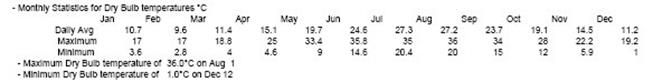
\includegraphics[width=0.9\textwidth, height=0.9\textheight, keepaspectratio=true]{media/image008.jpg}
\caption{Monthly Dry Bulb Data in SpreadSheet (for graphing) \protect \label{fig:monthly-dry-bulb-data-in-spreadsheet-for}}
\end{figure}

And these can be easily used to produce graphs:

\begin{figure}[hbtp] % fig 13
\centering
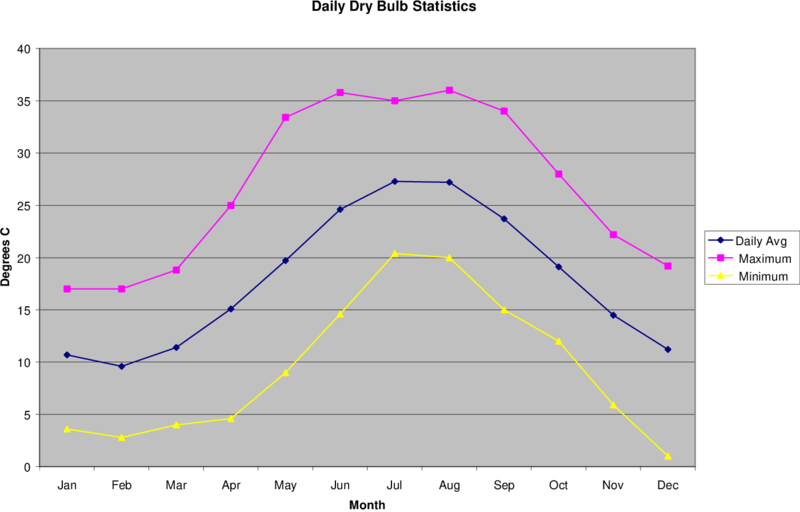
\includegraphics[width=0.9\textwidth, height=0.9\textheight, keepaspectratio=true]{media/image009.png}
\caption{Graph of Spreadsheet Data \protect \label{fig:graph-of-spreadsheet-data}}
\end{figure}

\subsection{Design Day Calculations Output}\label{design-day-calculations-output}

Using the WMO field (or determining it from the WBAN field), the Weather Converter performs table look up in the Design Condition files to see if there are recorded design conditions for the subject location. If this location is found, then design day objects are produced on the resultant design day object (ddy extension) file - ready for inclusion into an EnergyPlus input data file. If no design conditions are located, then the design day object file will still include a location object for inclusion with EnergyPlus. However, statistics using the weather file are displayed to the statistics file - these ``can'' be used to create your own design day definitions but you should read the warning that is issued and take care if your weather file is only a ``single instance'' weather data representation.

The location objects as well as the design condition objects are constrained by the data source. Some data sources do not have elevation information - thus, a location object from such a source will have an elevation of 0.0. Likewise, the time zone of some locations may not be available from the source data nor other data resources that the weather converter uses. A time zone will be estimated from the standard meridian of the location (determined by the longitude) but it may not be accurate. A user needs to be aware of these limitations when taking the design day files from the weather converter.

Note that you can always include a ``def'' file with this data to assure accuracy regardless of input format limitations.

An excerpt of a design day output is shown in the following (actual design day objects have been deleted for brevity). Note that with the 2009 ASHRAE HOF climate conditions, a possible DaylightSavingPeriod object may be included.

\begin{lstlisting}

! The following Location and Design Day data are produced as possible from the indicated data source.
  ! Wind Speeds follow the indicated design conditions rather than traditional values (6.7 m/s heating, 3.35 m/s cooling)
  ! No special attempts at re-creating or determining missing data parts (e.g. Wind speed or direction)
  ! are done.  Therefore, you should look at the data and fill in any incorrect values as you desire.


  Site:Location,
  Chicago Ohare Intl Ap_IL_USA Design_Conditions,     !- Location Name
  41.98,     !- Latitude {N+ S-}
  -87.92,     !- Longitude {W- E+}
  -6.00,     !- Time Zone Relative to GMT {GMT+/-}
  201.00;     !- Elevation {m}


  !  WMO = 725300 Time Zone = NAC: (GMT-06:00) Central Time (US & Canada)
  !  Data Source = ASHRAE 2009 Annual Design Conditions
  RunPeriodControl:DaylightSavingTime,
  2nd Sunday in March,    !- StartDate
  2nd Sunday in November;    !- EndDate


  ! Using Design Conditions from "Climate Design Data 2009 ASHRAE Handbook"
  ! Chicago Ohare Intl Ap_IL_USA Extreme Annual Wind Speeds, 1% = 11.1m/s, 2.5% = 9.4m/s, 5% = 8.6m/s
  ! Chicago Ohare Intl Ap_IL_USA Extreme Annual Temperatures, Max Drybulb = -23.7&deg;C Min Drybulb = 35.9&deg;C


  ! Chicago Ohare Intl Ap_IL_USA Annual Heating Design Conditions Wind Speed = 4.9m/s Wind Dir = 270
  ! Chicago Ohare Intl Ap Annual Cooling Design Conditions Wind Speed = 5.2m/s Wind Dir = 230

  ! Coldest Month = January
  ! Chicago Ohare Intl Ap IL USA Annual Heating 99.6%, MaxDB = -20&deg;C


  ! Chicago Ohare Intl Ap IL USA Annual Heating 99%, MaxDB = -16.6&deg;C


  ! Chicago Ohare Intl Ap IL USA Annual Cooling (DB = >MWB) 1%, MaxDB = 31.6&deg;C MWB = 23&deg;C


  ! Chicago Ohare Intl Ap IL USA Annual Humidification 99.6% Design Conditions DP = >MCDB, DP = -25.7&deg;C


  ! Chicago Ohare Intl Ap IL USA Annual Humidification 99% Design Conditions DP = >MCDB, DP = -22.1&deg;C


  ! Chicago Ohare Intl Ap IL USA Annual Heating Wind 99.6% Design Conditions WS = >MCDB, WS = 12.4m/s


  ! Chicago Ohare Intl Ap IL USA Annual Heating Wind 99% Design Conditions WS = >MCDB, WS = 11.4m/s




  ! Hottest Month = July
  ! Chicago Ohare Intl Ap IL USA Annual Cooling (DB = >MWB) .4%, MaxDB = 33.3&deg;C MWB = 23.7&deg;C


  ! Chicago Ohare Intl Ap IL USA Annual Heating Design Conditions Wind Speed = 4.9m/s Wind Dir = 270


  ! Chicago Ohare Intl Ap IL USA Annual Cooling (DB = >MWB) 2%, MaxDB = 30.1&deg;C MWB = 22.1&deg;C


  ! Chicago Ohare Intl Ap IL USA Annual Cooling (WB = >MDB) .4%, MDB = 31.2&deg;C WB = 25.5&deg;C


  ! Chicago Ohare Intl Ap IL USA Annual Cooling (WB = >MDB) 1%, MDB = 29.6&deg;C WB = 24.5&deg;C


  ! Chicago Ohare Intl Ap IL USA Annual Cooling (WB = >MDB) 2%, MDB = 28.1&deg;C WB = 23.5&deg;C


  ! Chicago Ohare Intl Ap IL USA Annual Cooling (DP = >MDB) .4%, MDB = 28.9&deg;C DP = 23.8&deg;C HR = 0.0192


  ! Chicago Ohare Intl Ap IL USA Annual Cooling (DP = >MDB) 1%, MDB = 27.7&deg;C DP = 22.9&deg;C HR = 0.0180


  ! Chicago Ohare Intl Ap IL USA Annual Cooling (DP = >MDB) 2%, MDB = 26.5&deg;C DP = 21.9&deg;C HR = 0.0170


  ! Chicago Ohare Intl Ap IL USA Annual Cooling (Enthalpy = >MDB) .4%, MDB = 31.4&deg;C Enthalpy = 79.2kJ/kg


  ! Chicago Ohare Intl Ap IL USA Annual Cooling (Enthalpy = >MDB) 1%, MDB = 29.6&deg;C Enthalpy = 75.1kJ/kg


  ! Chicago Ohare Intl Ap IL USA Annual Cooling (Enthalpy = >MDB) 2%, MDB = 28.2&deg;C Enthalpy = 70.9kJ/kg
\end{lstlisting}

Design day ``definitions'' originate in the ASHRAE Handbook of Fundamentals. Prior to 1997, these conditions were described for winter and summer (heating and cooling). They were based on seasonal percentages.

EnergyPlus uses the design day object values and creates an entire day of weather data - this is described more fully in the Input Output Reference under the \textbf{DesignDay} object. The weather converter program assigns ``SummerDesignDay'' and ``WinterDesignDay'' day types by default - these day types influence ``scheduling'' of various elements. How to use these effectively is described during the \textbf{DesignDay} and \textbf{Schedule} objects discussions in the Input Output Reference.

Beginning in 1997, and continuing (the latest version was published in 2009), the design condition data is based on annual percentages. In addition, only locations with long-term hourly observations data (on which to form the basis) are included.

\subsubsection{{[}From ASHRAE Handbook of Fundamentals, 2009{]}:}\label{from-ashrae-handbook-of-fundamentals-2009}

Design data based on dry-bulb temperature represent peak occurrences of the sensible component of ambient outdoor conditions. Design values based on wet-bulb temperature are related to the enthalpy of the outdoor air. Conditions based on dew point relate to the peaks of the humidity ratio. The designer, engineer, or other user must decide which set(s) of conditions and probability of occurrence apply to the design situation under consideration.

The 99.6\% and 99\% Heating conditions are often used in the sizing of heating equipment.

The 0.4, 1.0, and 2.0\% dry-bulb temperatures and mean coincident wet-bulb temperatures (i.e., DB = \textgreater{}MWB) often represent conditions on hot, mostly sunny days. These are often used in sizing cooling equipment such as chillers or air-conditioning units.

Design conditions based on wet-bulb temperatures (i.e., WB = \textgreater{}MDB) represent extremes of the total sensible plus latent heat of outdoor air. This information is useful for cooling towers, evaporative coolers, and fresh air ventilation system design.

Design conditions based on dew-point temperatures (i.e., DP = \textgreater{}MDB) are directly related to extremes of humidity ratio, which represent peak moisture loads from the weather. Extreme dew-point conditions may occur on days with moderate dry-bulb temperatures, resulting in high relative humidity. These values are especially useful for humidity control applications, such as desiccant cooling and dehumidification, cooling-based dehumidification, and fresh-air ventilation systems. The values are also used as a check point when analyzing the behavior of cooling systems at part-load conditions, particularly when such systems are used for humidity control as a secondary function. Humidity ratio values are calculated from the corresponding dew-point temperature and the standard pressure at the location's elevation.

The enthalpy design conditions (i.e.~Enthalpy = \textgreater{} MDB) gives the annual enthalpy for the cooling season; this is used for calculating cooling loads caused by infiltration and/or ventilation into buildings. Enthalpy represents the total heat content of air (the sum of its sensible and latent energies). Cooling loads can be easily calculated knowing the conditions of both the outdoor ambient and the building's interior air.
